%!TEX TS-program = xelatex
\documentclass[xetex,10pt,aspectratio=43]{beamer} 
%设置为 Beamer 文档类型,设置字体为 10pt,长宽比为16:9,数学字体为 serif 风格
\batchmode

\usefonttheme{professionalfonts}
\usetheme{Berlin} %主题
\usecolortheme{sustech} %主题颜色

\usepackage[UTF8]{ctex}
\usepackage{unicode-math}
\usepackage{graphicx}
\usepackage{animate}
\usepackage{tikz}
\usepackage{hyperref}

%导入一些用到的宏包
\usepackage{amsmath,bm,amssymb,enumerate,epsfig,bbm,calc,color,ifthen,capt-of,multimedia}
\usepackage[ruled,linesnumbered]{algorithm2e}

\usepackage{fancybox}
\usepackage{xcolor}
\usepackage{times}
\usepackage{listings}

\usepackage{booktabs}
\usepackage{colortbl}

\newcommand{\Console}{Console}
\lstset{ %
	backgroundcolor=\color{white},   % choose the background color
	basicstyle=\footnotesize\rmfamily,     % size of fonts used for the code
	columns=fullflexible,
	breaklines=true,                 % automatic line breaking only at whitespace
	captionpos=b,                    % sets the caption-position to bottom
	tabsize=4,
	commentstyle=\color{mygreen},    % comment style
	escapeinside={\%*}{*)},          % if you want to add LaTeX within your code
	keywordstyle=\color{blue},       % keyword style
	stringstyle=\color{mymauve}\ttfamily,     % string literal style
	numbers=left, 
	%	frame=single,
	rulesepcolor=\color{red!20!green!20!blue!20},
	% identifierstyle=\color{red},
	language=c
}

\setmathfont{XITS Math}

\definecolor{mygreen}{rgb}{0,0.6,0}
\definecolor{mymauve}{rgb}{0.58,0,0.82}
\definecolor{mygray}{gray}{.9}
\definecolor{mypink}{rgb}{.99,.91,.95}
\definecolor{mycyan}{cmyk}{.3,0,0,0}

%题目,作者,学校,日期
\title{离散数学基础}
\subtitle{\fontsize{9pt}{14pt}\textbf{集合运算}}
\author{中山大学MOOC课程组}
\institute{\fontsize{8pt}{14pt}中山大学计算机学院}
\date{\today}

%学校Logo
%\pgfdeclareimage[height=0.5cm]{sustech-logo}{sustech-logo.pdf}
%\logo{\pgfuseimage{sustech-logo}\hspace*{0.3cm}}

\AtBeginSection[]
{
	\begin{frame}<beamer>
		\frametitle{\textbf{目录}}
		\tableofcontents[currentsection]
	\end{frame}
}
\beamerdefaultoverlayspecification{<+->}

%图片
\graphicspath{{img/}}

%幂集
\newcommand{\powerset}{\raisebox{.15\baselineskip}{\ensuremath{\wp}}}
% -----------------------------------------------------------------------------
\begin{document}
	% -----------------------------------------------------------------------------
	
	\frame{\titlepage}
	
	\section[目录]{}   %目录
	\begin{frame}{目录}
		\tableofcontents
	\end{frame}

	\section{基本知识回顾}
	
	\begin{frame}{集合交}
		
		集合$A$,$B$的\textcolor{red}{交},记为$A\cap B$。
		
		$$A\cap B=\{x|x\in A\wedge x\in B\}$$
		
		\begin{columns}
			
			\begin{column}<1>{0.5\textwidth}
				
				\begin{figure}
					
					\centering
					
					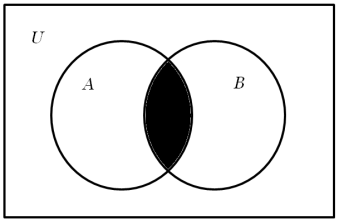
\includegraphics[scale=0.5]{9.png}
					
					\caption{集合$A\cap B$的文氏图}
					
				\end{figure}
			
			\end{column}
		
			\begin{column}<1>{0.5\textwidth}
				
				\begin{table}
				
					\centering
					
					\begin{tabular}{|c|c|c|}
						\hline
						$A$ & $B$ & $A\cap B$\\
						\hline
						0 & 0 & 0\\
						\hline
						0 & 1 & 0\\
						\hline
						1 & 0 & 0\\
						\hline
						1 & 1 & 1\\
						\hline
					\end{tabular}
					
					\caption{集合$A\cap B$的成员关系表}
				
				\end{table}
			
			\end{column}
		
		\end{columns}
			
	\end{frame}

	\begin{frame}{广义交}
		
		设$A$是一个集合族,即它的元素也是集合。它的\textcolor{red}{广义交},记为$\bigcap A$。
		
		$$\bigcap A=\{x|\forall S\subseteq A(x\in S)\}$$
		
	\end{frame}

	\begin{frame}{集合并}
	
		集合$A$,$B$的\textcolor{red}{并},记为$A\cup B$。
		
		$$A\cup B=\{x|x\in A\vee x\in B\}$$
	
		\begin{columns}
		
			\begin{column}<1>{0.5\textwidth}
			
				\begin{figure}
					
					\centering
					
					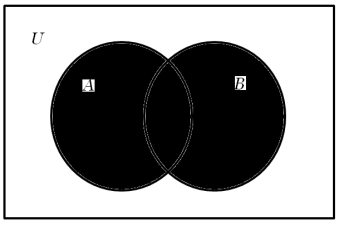
\includegraphics[scale=0.5]{1.png}
					
					\caption{集合$A\cup B$的文氏图}
				
				\end{figure}
			
			\end{column}
		
			\begin{column}<1>{0.5\textwidth}
			
				\begin{table}
				
					\centering
				
					\begin{tabular}{|c|c|c|}
						\hline
						$A$ & $B$ & $A\cup B$\\
						\hline
						0 & 0 & 0\\
						\hline
						0 & 1 & 1\\
						\hline
						1 & 0 & 1\\
						\hline
						1 & 1 & 1\\
						\hline
					\end{tabular}
				
					\caption{集合$A\cup B$的成员关系表}
				
				\end{table}
			
			\end{column}
		
		\end{columns}
	
	\end{frame}	

	\begin{frame}{广义并}
		
		集合$A$的\textcolor{red}{广义并},记为$\bigcup A$。
		
		$$\bigcup A=\{x|\exists S\subseteq A(x\in S)\}$$
		
	\end{frame}

	\begin{frame}{集合差}
	
		集合$A$,$B$的\textcolor{red}{差},记为$A-B$。
		
		$$A-B=\{x|x\in A\wedge x\notin B\}$$
		
		\begin{columns}
			
			\begin{column}<1>{0.5\textwidth}
				
				\begin{figure}
					
					\centering
					
					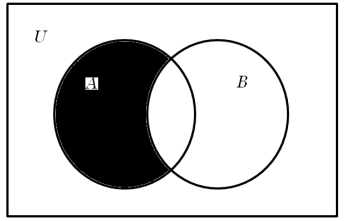
\includegraphics[scale=0.5]{7.png}
					
					\caption{集合$A-B$的文氏图}
					
				\end{figure}
				
			\end{column}
			
			\begin{column}<1>{0.5\textwidth}
				
				\begin{table}
					
					\centering
					
					\begin{tabular}{|c|c|c|}
						\hline
						$A$ & $B$ & $A-B$\\
						\hline
						0 & 0 & 0\\
						\hline
						0 & 1 & 0\\
						\hline
						1 & 0 & 1\\
						\hline
						1 & 1 & 0\\
						\hline
					\end{tabular}
					
					\caption{集合$A-B$的成员关系表}
					
				\end{table}
				
			\end{column}
			
		\end{columns}
		
	\end{frame}	

	\begin{frame}{集合补}
	
		集合$U$,$A$的\textcolor{red}{差}称为$A$的\textcolor{red}{补},记为$\overline{A}$。
		
		$$\overline{A}=\{x|x\in U\wedge x\notin A\}=\{x|x\notin A\}$$
		
		\begin{columns}
			
			\begin{column}<1>{0.5\textwidth}
				
				\begin{figure}
					
					\centering
					
					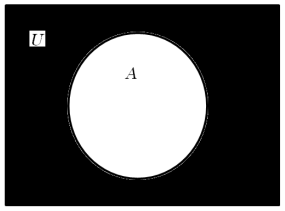
\includegraphics[scale=0.5]{41.png}
					
					\caption{集合$\overline{A}$的文氏图}
					
				\end{figure}
				
			\end{column}
			
			\begin{column}<1>{0.5\textwidth}
				
				\begin{table}
					
					\centering
					
					\begin{tabular}{|c|c|}
						\hline
						$A$ & $\overline{A}$\\
						\hline
						0 & 1\\
						\hline
						1 & 0\\
						\hline
					\end{tabular}
					
					\caption{集合$\overline{A}$的成员关系表}
					
				\end{table}
				
			\end{column}
			
		\end{columns}
		
	\end{frame}

	\begin{frame}{集合的幂集}
		
		集合$A$的所有子集构成的集合称为$A$的\textcolor{red}{幂集},记为$\powerset(A)$。$n$个元素的集合,它的幂集有$2^n$个元素。
		
		$$\powerset(A)=\{S|S\subseteq A\}$$
		
		\begin{block}<1>{例子}
			
			$A=\{1,2,3\}$
			
			$\powerset(A)=\{\varnothing,\{1\},\{2\},\{3\},\{1,2\},\{2,3\},\{1,3\},\{1,2,3\}\}$
		\end{block}
		
	\end{frame}
		
	\begin{frame}{定理}
		
		\begin{block}<1>{集合交满足交换律,$A\cap B=B\cap A$}
			
			$x\in A\cap B$当且仅当$x\in A\wedge x\in B$
			
			$x\in A\cap B$当且仅当$x\in B\wedge x\in A$
			
			$x\in A\cap B$当且仅当$x\in B\cap A$
			
		\end{block}
	
		\begin{block}<1>{集合交满足结合律,$A\cap (B\cap C)=(A\cap B)\cap C$}
			
			$x\in A\cap(B\cap C)$当且仅当$x\in A\wedge x\in B\cap C$
			
			$x\in A\cap(B\cap C)$当且仅当$x\in A\wedge x\in B\wedge x\in C$
			
			$x\in A\cap(B\cap C)$当且仅当$x\in A\cap B\wedge x\in C$
			
			$x\in A\cap(B\cap C)$当且仅当$x\in(A\cap B)\cap C$
			
		\end{block}
		
		\begin{block}<1>{集合交满足幂等律,$A\cap A=A$}
		
			$x\in A\cap A$当且仅当$x\in A\wedge x\in A$
			
			$x\in A\cap A$当且仅当$x\in A$
		
		\end{block}
	
	\end{frame}

	\begin{frame}{定理}
		
		\begin{block}<1>{对于任意集合$A$,$B$,$A\cap B\subseteq A$且$A\cap B\subseteq B$}
			
			$x\in A\cap B=x\in A\wedge x\in B\rightarrow x\in A$
			
			$x\in A\cap B=x\in A\wedge x\in B\rightarrow x\in B$
			
		\end{block}
	
		\begin{block}<1>{对于任意集合$A$,$B$,$C$,$C\subseteq A\cap B$当且仅当$C\subseteq A$且$C\subseteq B$}
			
			\begin{itemize}
				
				\item<1>必要性:$x\in C\rightarrow x\in A\cap B=x\in A\wedge x\in B$
				
				\item<1>充分性:$x\in C\rightarrow x\in A\wedge x\in B=x\in A\cap B$
				
			\end{itemize}
			
		\end{block}
	
	\end{frame}

	\begin{frame}{定理}
	
		\begin{block}<1>{集合并满足交换律,$A\cup B=B\cup A$}
			
			$x\in A\cup B$当且仅当$x\in A\vee x\in B$
			
			$x\in A\cup B$当且仅当$x\in B\vee x\in A$
			
			$x\in A\cup B$当且仅当$x\in B\cup A$
			
		\end{block}
		
		\begin{block}<1>{集合并满足结合律,$A\cup (B\cup C)=(A\cup B)\cup C$}
			
			$x\in A\cup(B\cup C)$当且仅当$x\in A\vee x\in B\cup C$
			
			$x\in A\cup(B\cup C)$当且仅当$x\in A\vee x\in B\vee x\in C$
			
			$x\in A\cup(B\cup C)$当且仅当$x\in A\cup B\vee x\in C$
			
			$x\in A\cup(B\cup C)$当且仅当$x\in(A\cup B)\cup C$
			
		\end{block}
		
		\begin{block}<1>{集合并满足幂等律,$A\cup A=A$}
			
			$x\in A\cup A$当且仅当$x\in A\vee x\in A$
			
			$x\in A\cup A$当且仅当$x\in A$
			
		\end{block}
		
	\end{frame}
	
	\begin{frame}{定理}
		
		\begin{block}<1>{对于任意集合$A$,$B$,$A\subseteq A\cup B$且$B\subseteq A\cup B$}
			
			$x\in A\rightarrow x\in A\vee x\in B=x\in A\cup B$
			
			$x\in B\rightarrow x\in A\vee x\in B=x\in A\cup B$
			
		\end{block}
		
		\begin{block}<1>{对于任意集合$A$,$B$,$C$,$A\cup B\subseteq C$当且仅当$A\subseteq C$且$B\subseteq C$}
			
			\begin{itemize}
				
				\item<1>必要性:
				
				$x\in A\cup B\rightarrow x\in C$
				
				$x\in A\vee x\in B\rightarrow x\in C$
				
				$x\in A\rightarrow x\in C$
				
				$x\in B\rightarrow x\in C$
				
				\item<1>充分性:
				
				$x\in A\rightarrow x\in C$
				
				$x\in B\rightarrow x\in C$
				
				$x\in A\vee x\in B\rightarrow x\in C$
				
				$x\in A\cup B\rightarrow x\in C$
			\end{itemize}
			
		\end{block}
		
	\end{frame}

	\begin{frame}{定理}
		
		\begin{block}<1>{对任意集合$A$和$B$,$A-B=A\cap\overline{B}$}
			
			$x\in A-B$当且仅当$x\in A\wedge x\notin B$
			
			$x\in A-B$当且仅当$x\in A\wedge x\in\overline{B}$
			
			$x\in A-B$当且仅当$x\in A\cap\overline{B}$
			
		\end{block}
	
		\begin{block}<1>{对任意集合$A$,$\overline{\overline{A}}=A$}
			
			$x\in \overline{\overline{A}}$当且仅当$x\notin \overline{A}$
			
			$x\in \overline{\overline{A}}$当且仅当$x\in A$
			
		\end{block}
		
	\end{frame}

	\begin{frame}{定理}
		
		\begin{block}<1>{对任意两个集合$A$,$B$,$\overline{A\cap B}=\overline{A}\cup\overline{B}$}
			
			$x\in\overline{A\cap B}$当且仅当$x\notin A\cap B$
			
			$x\in\overline{A\cap B}$当且仅当$\lnot(x\in A\cap B)$
			
			$x\in\overline{A\cap B}$当且仅当$\lnot(x\in A\wedge x\in B)$
			
			$x\in\overline{A\cap B}$当且仅当$x\notin A\vee x\notin B$
			
			$x\in\overline{A\cap B}$当且仅当$x\in\overline{A}\vee x\in \overline{B}$
			
			$x\in\overline{A\cap B}$当且仅当$x\in\overline{A}\cup \overline{B}$
			
		\end{block}
	
		\begin{block}<1>{对任意两个集合$A$,$B$,$\overline{A\cup B}=\overline{A}\cap\overline{B}$}
			
			$x\in\overline{A\cup B}$当且仅当$x\notin A\cup B$
			
			$x\in\overline{A\cup B}$当且仅当$\lnot(x\in A\cup B)$
			
			$x\in\overline{A\cup B}$当且仅当$\lnot(x\in A\vee x\in B)$
			
			$x\in\overline{A\cup B}$当且仅当$x\notin A\wedge x\notin B$
			
			$x\in\overline{A\cup B}$当且仅当$x\in\overline{A}\wedge x\in\overline{B}$
			
			$x\in\overline{A\cup B}$当且仅当$x\in\overline{A}\cap\overline{B}$
			
		\end{block}
	
	\end{frame}

	\begin{frame}{定理}
		
		\begin{block}<1>{对任意两个集合$A$,$B$,$A-B\subseteq A$}
			
			$x\in A-B=x\in A\cap\overline{B}=x\in A\wedge x\in\overline{B}\rightarrow x\in A$
			
		\end{block}
	
		\begin{block}<1>{对任意两个集合$A$,$B$,$A\subseteq B$当且仅当$\overline{B}\subseteq\overline{A}$}
			
			\begin{itemize}
				
				\item<1>必要性:
				若$x\in \overline{B}$且$x\notin \overline{A}$,则$x\notin B$且$x\in A$。
				
				由$A\subseteq B$,有$x\in B$,矛盾。
				
				\item<1>充分性:
				若$x\in A$且$x\notin B$,则$x\in \overline{B}$。
				
				由$\overline{B}\subseteq\overline{A}$,有$x\in\overline{A}$,有$x\notin A$,矛盾。
				
			\end{itemize}
		
		\end{block}
	
	\end{frame}

	\begin{frame}{定理}
		
		\begin{block}<1>{对任意两个集合$A$,$B$,$A\subseteq B$当且仅当$A-B=\varnothing$}
			
			\begin{itemize}
				
				\item<1>必要性:
				若$\exists x\in A-B$,有$x\in A\cap\overline{B}$,有$x\in A\wedge x\in\overline{B}$,有$x\notin B$。
				
				由$A\subseteq B$,有$x\in B$,矛盾。
				
				\item<1>充分性:
				若$x\in A$且$x\notin B$,有$x\in A\wedge x\in\overline{B}$,有$x\in A\cap\overline{B}$,有$x\in A-B$,有$x\in\varnothing$,矛盾。
				
			\end{itemize}
		
		\end{block}
	
	\end{frame}

	\begin{frame}{定理}
		
		\begin{block}<1>{幂集运算保持子集关系,$A\subseteq B\rightarrow\powerset(A)\subseteq\powerset(B)$}
			
			$X\in\powerset(A)=X\subseteq A$
			
			$A\subseteq B\rightarrow X\subseteq B=X\in\powerset(B)$	
						
		\end{block}
	\end{frame}

	\begin{frame}[fragile]{幂集计算的算法}
		
		当全集$U$有$n$个元素时,它的每个子集$A$都可用一个长度为$n$的二进制字符串表示
		
		串的每一位对应一个元素,第$i$位对应元素$a_i$,第$i$位为1时,表示$a_i\in A$,第$i$位为0时,表示$a_i\notin A$
		
	\end{frame}

	\begin{frame}[fragile]{幂集计算的算法}
			
		\begin{columns}
			
			\begin{column}<1>{0.5\textwidth}
			
			根据定义,$U$的幂集的计算,就是计算$U$的所有子集。$U$一共有$2^n$个子集,用二进制表示就是从$0$到$2^n-1$。我们只需要让二进制串从$0$每次递增$1$,直到$2^n-1$。
			
			程序的初始状态为$0$,终止状态为$2^n-1$。每个状态表示一种结果。
			
			如何实现递增?考虑二进制加法,$0+1=1$,$1+1=10$。若我们所加的位$b_i$为$0$,我们将它改为$1$即可。若$b_i$为$1$,我们需要将$b_i$改为$0$,向下一位加$1$。
			
			\end{column}
			
			\begin{column}<1>{0.5\textwidth}
				
				\begin{figure}
				
					\centering
					
					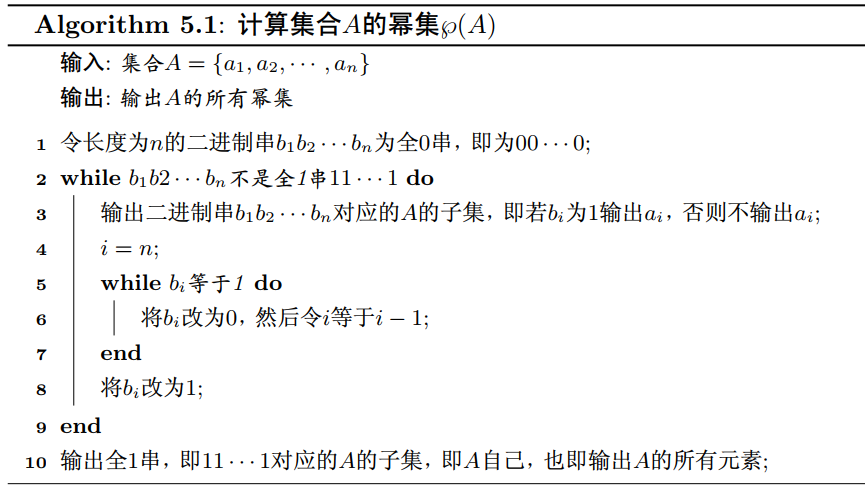
\includegraphics[scale=0.3]{01.png}
					
				\end{figure}	
					
			\end{column}
			
		\end{columns}

	\end{frame}

	\section{习题讲解}
	
	\begin{frame}{计算$A\cap B$,$A\cup B$和$A−B$}
		
	设全集$U$是自然数集,集合$A$和$B$都是全集$U$的子集,且$A=\{3k|k\in N\}$,$B=\{4k|k\in N\}$
	
	因为$N=\{k|\exists z\in N(k=4z\vee k=4z+1\vee k=4z+2\vee k=4z+3)\}$
	
	所以$3|x\leftrightarrow x=3k=12z\vee 12z+3\vee 12z+6\vee 12z+9$
	
	同理$4|x\leftrightarrow x=4k=12z\vee 12z+4\vee 12z+8$
	
	因为$x\in A\cap B\leftrightarrow x\in A\wedge x\in B\leftrightarrow 3|x\wedge 4|x\leftrightarrow 12|x$
	
	所以$A\cap B=\{12k|k\in N\}$
	
	因为$x\in A\cup B\leftrightarrow x\in A\vee x\in B\leftrightarrow 3|x\vee 4|x$
	
	所以$A\cup B=\{x|\exists k\in N(x=12k\vee x=12k+3\vee x=12k+4\vee x=12k+6\vee x=12k+8\vee x=12k+9)\}$
	
	因为$x\in A-B\leftrightarrow x\in A\cap\overline{B}\leftrightarrow x\in A\wedge x\in\overline{B}\leftrightarrow x\in A\wedge x\notin B$

	所以$A-B=\{x|\exists k\in N(x=12k+3\vee x=12k+6\vee x=12k+9)\}$

	\end{frame}

	\begin{frame}{计算$A\cap B$,$A\cup B$和$A−B$}
		
		\textcolor{mymauve}{集合运算,首先要搞清楚$A$和$B$的元素情况,如果元素数量较少,可用枚举法表示集合$A$和$B$,再进行运算\\
		如果元素较多,需要使用描述法表示集合,通常将集合的运算转化成逻辑的运算}
	
	\end{frame}
	
	\begin{frame}{计算$\bigcap A$和$\bigcup A$}
		
	设$A_n$是$n$的所有正因子构成的集合,集合族$A=\{A_{4k}|k\in Z^{+}\}$
	
	易知$A_4=\{1,2,4\}$,同时1,2,4还是4k(任意$k\in Z^{+}$)的因子
	
	故有$\bigcap A={1,2,4}$	
	
	易知对任意$k\in Z^{+}$,k是4k的因子
	
	故有$\bigcup A=Z^{+}$

	\textcolor{mymauve}{求集合族的广义交和广义并,需要考虑每个集合的元素,所有集合所共有的元素是集合族广义交的元素,所有集合的元素是集合族广义并的元素\\
	广义交优先考虑特例,从较少元素的集合入手,用的是排除的策略,不断减少元素\\
	广义并就要多考虑有没有漏掉的元素,用的是补充的策略,不断增加元素}
		
	\end{frame}
	
	\begin{frame}{计算幂集}
	
	\begin{block}<1>{$\{\varnothing,\{\varnothing\}\}$}
		
		集合中的元素有:$\varnothing$,$\{\varnothing\}$
		
		集合的子集:$\varnothing$,$\{\varnothing\}$,$\{\{\varnothing\}\}$,$\{\varnothing,\{\varnothing\}\}$
		
		集合的幂集:$\{\varnothing,\{\varnothing\},\{\{\varnothing\}\},\{\varnothing,\{\varnothing\}\}\}$
		
	\end{block}

	\begin{block}<1>{$\powerset(\{\{a\}\})$}
		
		令$A=\{\{a\}\}$
		
		$A$的元素:$\{a\}$
		
		$A$的子集:$\varnothing$,$\{\{a\}\}$
		
		$\powerset(A)$:$\{\varnothing,\{\{a\}\}\}$
		
		令$B=\powerset(A)$
		
		$B$的元素:$\varnothing$,$\{\{a\}\}$
		
		$B$的子集:$\varnothing$,$\{\varnothing\}$,$\{\{\{a\}\}\}$,$\{\varnothing,\{\{a\}\}\}$
		
		$\powerset(B)$:$\{\varnothing,\{\varnothing\},\{\{\{a\}\}\},\{\varnothing,\{\{a\}\}\}\}$
	\end{block}
			
	\end{frame}

	\begin{frame}{计算幂集}
			
		\textcolor{mymauve}{计算幂集可分为三步,先列出所有元素,再将元素组合成子集,将子集作为幂集的元素\\
		求子集时,不要忘了空集}
	
	\end{frame}

	\begin{frame}{判断命题真值}
		
	\begin{block}<1>{$\{a\}\in\{a,\{a\}\}$}
		
		符号是$\in$,判断元素是否属于集合
		
		令$A=\{a,\{a\}\}$
		
		$A$的元素:$a$,$\{a\}$
		
		$\{a\}$是$A$的元素
		
		$\{a\}\in\{a,\{a\}\}$真值为1
		
	\end{block}

	\begin{block}<1>{$\{a\}\subseteq\{a,\{a\}\}$}
		
		符号是$\subseteq$,判断集合之间的关系
		
		令$A=\{a\}$,$B=\{a,\{a\}\}$
		
		$A$的元素:$a$
		
		$B$的元素:$a$,$\{a\}$
		
		$A$中的所有元素都属于$B$
		
		$\{a\}\subseteq\{a,\{a\}\}$真值为1
	\end{block}
		
	\textcolor{mymauve}{首先要看好符号$\in$,$\subseteq$,再将集合的元素列出来,根据定义即可}
	
	\end{frame}

	\begin{frame}{用文氏图表示集合表达式}
		
	\begin{columns}
		
		\begin{column}<1>{0.3\textwidth}
			
			$$A\cap(B\cup C)$$
			
			\begin{figure}
				
				\centering
				
				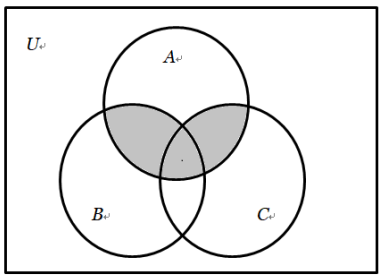
\includegraphics[scale=0.5]{4.png}
				
			\end{figure}
		
		\end{column}
		
		\begin{column}<1>{0.3\textwidth}
			
			$$A-(B\cup C)$$
			
			\begin{figure}
				
				\centering
				
				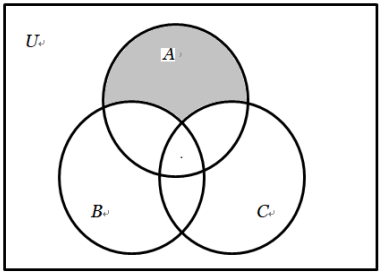
\includegraphics[scale=0.5]{17.png}
				
			\end{figure}	
			
		\end{column}
	
		\begin{column}<1>{0.3\textwidth}
		
			$$A-(B-C)$$
			
			\begin{figure}
				
				\centering
				
				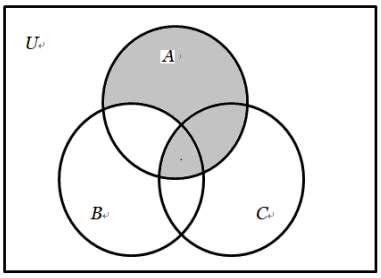
\includegraphics[scale=0.5]{21.png}
				
			\end{figure}	
			
		\end{column}
		
	\end{columns}

	\end{frame}

	\begin{frame}{用成员关系表表示集合表达式}
	
		\begin{table}
			
			\centering
			
			\begin{tabular}{|c|c|c|c|c|c|c|c|}
				\hline
				$A$ & $B$ & $C$ & $B\cup C$ & $B-C$ & $A\cap(B\cup C)$ & $A-(B\cup C)$ & $A-(B-C)$\\
				\hline
				0 & 0 & 0 & 0 & 0 & 0 & 0 & 0\\
				\hline
				0 & 0 & 1 & 1 & 0 & 0 & 0 & 0\\
				\hline
				0 & 1 & 0 & 1 & 1 & 0 & 0 & 0\\
				\hline
				0 & 1 & 1 & 1 & 0 & 0 & 0 & 0\\
				\hline
				1 & 0 & 0 & 0 & 0 & 0 & 1 & 1\\
				\hline
				1 & 0 & 1 & 1 & 0 & 1 & 0 & 1\\
				\hline
				1 & 1 & 0 & 1 & 1 & 1 & 0 & 0\\
				\hline
				1 & 1 & 1 & 1 & 0 & 1 & 0 & 1\\
				\hline
			\end{tabular}
			
		\end{table}	

	\end{frame}

	\section{总结}
	
	\begin{frame}{总结}
		
		本节要牢记各运算的定义,掌握计算和定理的证明
		
		\begin{itemize}
			
			\item<1> 集合的运算
			
			\item<1> 重要定理
			
		\end{itemize}
		
	\end{frame}
	
	\begin{frame}{Thank you}
		\begin{center}
			\begin{minipage}{\textwidth}
				\setbeamercolor{mybox}{fg=white, bg=black!50!blue}
				\begin{beamercolorbox}[wd=0.70\textwidth, rounded=true, shadow=true]{mybox}
					\LARGE \centering Thank you for listening!  %结束语
				\end{beamercolorbox}
			\end{minipage}
		\end{center}
	\end{frame}
	
	
	% -----------------------------------------------------------------------------
\end{document}
%文档结束
